\documentclass[a4paper]{article}

\usepackage[utf8]{inputenc}
\usepackage[T1]{fontenc}
\usepackage{lmodern}
\usepackage[ngerman]{babel}
\usepackage{amsmath}
%\usepackage[amssymb]{SIunits}
%\usepackage{sistyle}
%\SIstyle{German}
\usepackage{hyperref}
%\usepackage[square]{natbib}
%\usepackage{upgreek}
\usepackage{tikz}
\usepackage{pgfplots}
\pgfplotsset{width=11cm, height=7.5cm, compat=1.11}
%\pgfplotsset{compat=1.11}
\usepackage{float} % to use the [H] parameter in figures
\usepackage[margin=1cm, font=small, labelfont=bf]{caption} % caption margin
%\usepackage[left=4.5cm, right=4.5cm, top=2cm, bottom=2cm]{geometry}
\usepackage{graphicx}
\usepackage{cite}


\title{Versuche zur Optischen Informationsübertragung}
\author{Henrik Kröger \and Nicolás Pulido}
\date{Durchgeführt am 26. und 27. April 2016}

\begin{document}

\maketitle

%\noindent Einleitungstext

\tableofcontents

\newpage
\section{Faseroptische Übertragungsstrecke} 

%\subsection{lineare Dagradationen}

\subsection{Verluste}
Verluste im Faser bestimmen wie lang eine kontinuierliche Strecke sein kann
bevor man ein Verstärker benutzen muss. Es gibt in Glass prinzipiell drei
verschiedene Arten von Verlusten: \emph{Absorption}, \emph{Streuung}, und
\emph{Krümmungsverluste}. 


Absorption ist sehr klein und damit fast vernachlässigbar, in der Spektrum von
Wellenlängen die kommerziell benutzt werden, im Vergleich zu Krümmung und
Streuung. Es wird von Verunreinigungen verursacht.

\subsubsection{Streuung}

\begin{description}
  \item[Rayleigh Streuung:] Es wird aus Wechselwirkungen entstanden, des Lichts
    und Fluktuationen der Dichte, die während der Herstellung des Fasers
    verursacht werden. 

  \item[Brillouin Streuung:] Es wird von akustische Wellen induziert. 

  \item[Raman Streuung:] Es ist ein Effekt von molekulare Vibrationen von
    \emph{optische} Phononen, die von die Wechselwirkung von der Quarzmolekülen
    und einem starken Magnetfeld verursacht wird.
\end{description}

Brillouin und Raman Streuung sind \emph{nicht lineare} Effekte, die nur bei höhe
Leistungen auftreten. Dies kann ein Faktor, das Systeme mit hoher Leistung
begrenzt. 

%\paragraph{Dämpfung}
%\paragraph{Koppelverluste}


\subsubsection{Krümmungsverluste}
Wenn Verluste wegen Verunreinigungen fast ganz beseitigt sind, es
bleiben noch die Verluste, die wegen die eigentliche Struktur des Glases
verursacht sind.  Wenn der Krümmungsradius im Bereich der Zentimeter liegt,
spricht man von makroskopischen Krümmungsverluste. 
Bei eine Krümmung kann der kritische Winkel für die Totalreflexion
überschritten werden in der gebogenen Portion. 

Man musst für Multimodenfaser die wellenoptische Beschreibung benutzen. Die
Feldverteilung jeder Mode erstreckt sich auch in das Mantel. In der gekrümmten
Stelle des Fasers gibt es eine Stelle, gegen dem äußerem Teil der Kurve, wo die
Propagationsgeschwindigkeit fängt zu überschreiten, die im Medium durch den
Brechungsindex erlaubte Geschwindigkeit. Der Wellenfront wird effektiv nicht
mehr eben und daher zeigt ein Komponent des Poynting-Vektors nach außen, in
senkrechter Richtung zur Faser, was zur Energieverluste durch Radiation führt. 

Das Faser wird mechanisch am äußeren Teil der Kurve expandiert und am inneren
Teil komprimiert, was der Brechungsindex in dieser Regionen so verändert, dass 
die Verluste einigermaßen zu kompensiert werden, obwohl dies nicht genug ist um
die Verluste zu vermeiden.

Es ist klar: je weniger dringt der Feld im Mantel ein, desto weniger
Krümmungsverluste gibt es. 


\subsubsection{Chromatische Dispersion}
Ein Signal kann sich verzerren, während es sich durch einen optischen
Träger fortbewegt. Viele Arten dieser Verzerrungen passieren, weil
verschiedene Teile des Signals sich mit verschiedenen Geschwindigkeiten
bewegen. Es besteht die Gefahr, dass das Signal beim Empfänger so
stark verzerrt ankommt, dass er nicht mehr in der Lage ist, es zu
entschlüsseln. In \emph{Multimodenfasern} findet man:
\begin{description}
  \item[Modendispersion:] Jede Mode kann unterschiedlich
    tief in den Mantel der Faser eindringen und sich damit mit verschiedenen
    Geschwindigkeiten fortpflanzen.
\end{description} 
In \emph{Monomodenfaser} gibt es auch Dispersion. Der Grund
dafür ist, dass der Brechungsindex abhängig von der Wellenlänge ist.
Lichtpulse oder Wellenpakete haben immer eine gewisse spektrale Breite und die
verschiedenen Frequenzkomponenten des Pulses pflanzen sich dann mit
unterschiedlichen Geschwindigkeiten fort, was zu Verzerrungen des Pulses führt.
Man kann im Monomodenfaser folgende Dispersionsarten unterscheiden:
\begin{description}
  \item[Materialdispersion:] Dies ist eine direkte Konsequenz der
    Abhängigkeit des Brechungsindexes von der  Wellenlänge und es geschieht
    nicht nur in optischen Fasern, sondern auch in jedem Glas und ist unabhängig von
    der Geometrie der Faser.
  \item[Wellenleiterdispersion:] Der Lichtpuls propagiert auch im Mantel,
    der einen anderen Brechungsindex als der Kern hat. Wenn man die
    Wellenlänge variiert, gibt es einen Übergang zwischen Propagation,
    die meist im Kern und Propagation, die meist im Mantel stattfindet.
    Dies macht den effektiven Brechungsindex abhängig von der Wellenlänge.
  \item[Profildispersion:] Sie ist kleiner als die Moden- und
    Materialdispersion. Der Unterschied zwischen den Brechungsindexen von Kern
    und Mantel ist auch von der Wellenlänge abhängig.
  \item[Polarisationsmodendispersion:] Sie ist auch klein. Die Polarisation des
    Lichtes kann in zwei orthogonale Komponenten zerlegt werden. Der
    Brechungsindex von Glas ist streng genommen nicht ganz kreissymmetrisch,
    d.h. jedes Glas ist ein bisschen doppelbrechend. Verschiedene
    Brechungsindizes für jede Polarisationskomponente führen zur Dispersion.
\end{description}

%\subsection{Nicht-lineare Degradationen}
%\paragraph{Vierwellenmischung}
%\paragraph{Selbstphasenmodulation}
%\paragraph{Kreuzphasenmodulation}

\subsection{Versuch}
Es werden Übertragungsverluste an einem optischen Übertragungssystem
mithilfe von \emph{Optischer Zeitbereichsreflektometrie (OTDR)} und
einem Powermeter untersucht.
Die \emph{Rückstreukurve} soll durch unterschiedliche Fasertypen etc.
manipuliert werden.

\subsubsection{OTDR Einführung}
Mittels OTDR misst man die Dämpfung der Signal im Träger. Vorteile sind, dass
es eine zerstörungsfreie Messung ist, die \emph{in situ} an nur eine der Enden
des Fasers gemacht werden kann. Man bekommt damit Information über die
Abhängigkeit der Dämpfung von der Länge und über die Einfügedämpfung, womit man
inferieren kann, ob es Defekten, Spleißen, Biegungen oder Koppler sich im Faser
befinden, sowie die Lage desselben. Die Ortsauflösung der Messung ist eine
Faltung zwischen die Pulsbreite und die Antwortfunktion des Detektionssytems.  

\subsubsection{Funktionsprinzip} 
Das OTDR sendet Lichtpulse durch eine Ende des Fasers, und misst wieviel Zeit
passiert ist, bis die Lichtsignale zurückkommen.  Als die Pulse sich im Fiber
fortpflanzen, treffen sie streuende und reflektierende Stellen, was das Licht
zurück ins Apparat sendet. Die physikalische Ursachen davon sind
Rayleigh-Streuung und Fresnel-Reflexion.  Indem man die Ankunftszeit dieses
zurückkehrendes Licht misst, kann man die Position und Größe der Fehler im
Faser bestimmen.

Ein Pulsgenerator, der von einem digitalen Signalprozessor getriggert wird,
moduliert die Intensität eines Lasers. Typischerweise handelt es sich um ein
viereckiger Laserpuls mit eine Breite von 5 ns bis 10 $\mu$s. Ein
Richtkoppler leitet das Rückkehrende Signal in einem Photodetektor und wird
dann verstärkt, in einem ADC digitalisiert und im Signalprozessor analysiert.
Die Abtastrate des ADC bestimmt die räumliche Weite der Abtastwerten. Zum
Beispiel, eine Abtastrate von 50 Hz führt zu eine Räumliche Weite von 2 m. Um
die räumliche Weite zu verkleinern ist es in der Praxis günstiger, die
Abtastwerten von verschiedene Messungen zu mischen, als die Abtastfrequenz zu
erhöhen, in einem Prozess, der Interleaving genannt wird.

\subsubsection{Faser Spur}
Nach der Messung bekommt man eine Spur, die das Faser charakterisiert. Der
Graph wird folgendermassen interpretiert:
\begin{description}
  \item[$x$-Axis:] Zeigt die Distanz vom Messapparat der rückstreuende Stelle
    in m.
  \item[$y$-Axis:] Entspricht die Leistung in dB des Rückstreulichtes.
\end{description}
Es wird ein Umrechnungsfaktor von 
\begin{equation*}
1 \ \mathrm m = 10^{-8} \ \mathrm s 
\end{equation*}
benutzt um die Distanz aus der verstrichene Zeit anzugeben. Die
Lichtgeschwindigkeit im Faser ist
\begin{equation*}
  v = \frac{c}{n}, \quad\quad \text{mit } n = 1.5 \text{ für Quarzglas.}
\end{equation*}
Damit erhalten wir eine Geschwindigkeit im Medium von 
\begin{equation*}
  v = \frac{3 \cdot 10^{8}}{\frac{3}{2}} = 2 \cdot 10^{8}
  \ \frac{\mathrm m}{\mathrm s}.
\end{equation*} Das Licht braucht also $\frac{1}{2} 10^{-8}$ Sekunden um 1
Meter sich fortzupflanzen. Aber man misst eigentlich das doppelte Zeit, da man
die Zeit des Echos registriert. Damit ergibt sich der obige Umrechnungsfaktor
von $1\ \mathrm m = 10^{-8} \ \mathrm s$. Die Leistungsverluste am Detektor
müssen auch halbiert werden, denn sie die Verluste der Hin- und Rückweg
entsprechen. Daher werden die Werte im $y$-Axis, die in dB gegeben werden, mit
einem Faktor $5\log_{10}$ anstatt von $10\log_{10}$ berechnet.

Am Faser Spur erkennt man 3 verschiedene Arten von Features:
\begin{description}
  \item[gerade Linien:] Sind von der verteilte Rayleigh Streuung verursacht.
  \item[positive Spizen:] Sind von diskrete Reflexionen verursacht.
  \item[positive oder negative Stufen:] Entsprechen nicht-reflektierende
    Ereignisse. 
\end{description}

\emph{Nicht-reflektierende Ereignisse} deuten mechanische Biegungen des Fasers,
die Verluste durch dem Mantel verursachen, oder Schweiss Spleißen an. Sie
zeigen eine plötzliche Senkung der Rückstreuleistung. Im Fall von Spleißen,
wenn die gespleißten Fasern identisch waren, dann entspricht die Größe der
Stufe, die Einfügedämpfung des Spleißes. Wenn die gespleißte Fasern aber
verschieden waren, dann kann man nur die genaue Einfügedämpfung bekommen, indem
man der Mittelwert über zwei Messungen, je an eine der Enden des Fasers,
berechnet. 

\emph{Reflektierende Ereignisse} sind wegen Unterschiede der Brechungsindex,
die zur Fresnel-Reflexionen führen verursacht. Sie werden als Spitzen im
Rückstreukurve registriert. Diese Reflexionen können von mechanische Spleißen
verursacht werden oder von optische Stecker. In beiden Fällen sind kleine
Gebiete mit Luft im Faser gegeben, und damit ergibt sich beim Glas-Luft
Übergang eine Fresnel-Reflexion.

\subsubsection{Leistungsparameter}

Folgende Parameter, die man am Faserspur zu lesen sind, charakterisieren die
Messfähigkeit eines OTDRs:

\begin{description}
  \item[Dynamisches Bereich:] Es ist die Differenz zwischen der 
    Rückstreuleistung am Anfang und der Niveau des Rauschens.
 
  \item[Messbereich:] Es besagt die maximale Dämpfung eines Ereignisses, die
    noch Identifiziert werden kann.
  
  \item[Todeszonen:] Die sind immer mit reflektive Ereignisse verbunden. Das
    OTDR Apparatur wird von das Rückstreulicht der Reflexion saturiert und
    braucht einige Zeit um wieder empfindlich zu sein. Es gibt zwei Typen von
    Todeszonen: Die \emph{Ereignis Todeszone} ist der Abstand zwischen der
    Anfang der Reflexion und der 1.5 dB Punkt an der Fallende Ecke. Die
    \emph{Dämpfung Todeszone:} ist der Abstand zwischen der Anfang der
    Reflexion und der 0.5 dB Punkt vor der Ende des Schwanzes.
  
      \item[Räumliche Schärfe:] Entspricht die Fähigkeit, zwei
    nebeneinanderliegende Ereignisse zu unterscheiden.
\end{description}

\subsubsection{Messung}
Im Versuch wurde mit zwei verschiedene Pulsbreiten gemessen, und zwar 50 ns 
und 100 ns. In Abbildung \ref{fig:pw50} wird die Spur des Fasers dargestellt
, die mit eine Pulsbreite von 50 ns gemessen war. 
\begin{figure}[H]
  \centering
  \begin{tikzpicture}
    \begin{axis}[
	title = OTDR Messung Pulsweite $50\ \mathrm{ns}$,
	xlabel = Entfernung vom Detektor in m,
	ylabel = Leistung am Detektor in dB,
      ]
      %\addplot[samples=2] gnuplot[raw gnuplot]{plot 'messungen/OTDR_PW50.dat'};
      \addplot[
	samples=2,
      	] table {./messungen/OTDR_PW50.dat};
      \node[pin=45:Anfangsreflexion] at (59, 44.760) {};
      \node[pin=90:1. Spleiß] at (2046, 36.524) {};
      \node[pin=90:2. Spleiß] at (4028, 35.827) {};
      \node[pin=90:Stecker] at (5964, 36.023) {};
      \node[pin=90:Ende] at (8094, 35.294) {};
    \end{axis}
  \end{tikzpicture}
  \caption{Faser Spur gemessen mit eine Pulsbreite von 50 ns. Verschiedene
  erkennbare Ereignisse sind markiert. Es gibt keine Reflexion am Ende, da 
  dies mit Absicht unregelmäßig gebrochen war.}
  \label{fig:pw50}
\end{figure}

Aus der Faserspur berechnet man die Verluste indem man Geraden vor und nach dem
Ereignis fittet und den vertikalen Abstand rechnet. Im folgendem wird die
Berechnung der Verluste für den 1. und 2. Spleiß, sowie für den Stecker
durchgeführt und in Abbildungen \ref{fig:spl1}, \ref{fig:spl2} und
\ref{fig:steck1} graphisch dargestellt.

\begin{figure}[H]
  \centering
  \begin{tikzpicture}
    \begin{axis}[
	title = Verluste am 1. Spleiß,
	xlabel = Entfernung vom Detektor in m,
	ylabel = Leistung am Detektor in dB,
	xmin = 1800,
	xmax = 2400,
      ]
      \addplot[
      	samples=2,
      	%restrict x to domain=71:4050,
      	restrict x to domain=1800:2400,
	%only marks,
	%mark size=0.6pt,
     	] 
	table {./messungen/OTDR_PW50.dat};
      \addplot[samples=2, domain=1800:2200, thick] {3.67302974e+01 -1.14182000e-04*x};
      \addplot[samples=2, domain=2000:2400, thick] {3.59826848e+01 -6.51226945e-05*x};
      \draw[<->, thick] (2044.44, 36.497) -- (2044.44, 35.85);
      \draw (2044.44,  36.173) node[align=center, anchor=east]
      	{1. Spleiß Verlust\\= 0.647 dB};
      \node[pin=45:Position des Sipleißes] at (2044.44, 36.497) {};
    \end{axis}
  \end{tikzpicture}
  \caption{Messung der Verlust am 1. Spleiß. Es würde den Abstand zwischen zwei
  gefittete Geraden berechnet.}
  \label{fig:spl1}
\end{figure}

\begin{figure}[H]
  \centering
  \begin{tikzpicture}
    \begin{axis}[
	title = Verluste am 2. Spleiß,
	xlabel = Entfernung vom Detektor in m,
	ylabel = Leistung am Detektor in dB,
	xmin = 3800,
	xmax = 4300,
      ]
      \addplot[
      	samples=2,
      	restrict x to domain=3800:4300,
     	] 
	table {./messungen/OTDR_PW50.dat};
      \addplot[samples=2, domain=3000:4100, thick] {3.59826848e+01 -6.51226945e-05*x};
      \addplot[samples=2, domain=4025:5000, thick] {3.57670249e+01 -4.94830018e-05*x};
      \draw[<->, thick] (4038, 35.7196411674) -- (4038, 35.5672125844);
      \draw (4038,  35.65) -- (3975, 35.5) node[align=center, anchor=east]
      	{2. Spleiß Verlust\\= 0.152 dB};
      \node[pin=45:Position des Sipleißes] at (4038, 35.72) {};
    \end{axis}
  \end{tikzpicture}
  \caption{Messung der Verlust am 2. Spleiß. Wie oben, es würde den Abstand
  zwischen zwei gefittete Geraden berechnet.}
  \label{fig:spl2}
\end{figure}

\begin{figure}[H]
  \centering
  \begin{tikzpicture}
    \begin{axis}[
	title = Verluste am Stecker,
	xlabel = Entfernung vom Detektor in m,
	ylabel = Leistung am Detektor in dB,
	xmin = 5745,
	xmax = 6206,
      ]
      \addplot[
      	samples=2,
      	restrict x to domain=5745:6206,
     	] 
	table {./messungen/OTDR_PW50.dat};
      \addplot[samples=2, domain=5745:5975, thick] {3.57670249e+01
      -4.94830018e-05*x};
      \addplot[samples=2, domain=5925:6202, thick] {3.51381770e+01
      -8.71765157e-06*x};
      \draw[<->, thick] (5949, 35.4726505679) -- (5949, 35.0863157209);
      \draw (5949,  35.3) -- (5885, 35.1) node[align=center, anchor=east]
      	{Stecker Verlust\\= 0.386 dB};
	\draw[thick] (5949, 35.4726505679) -- (5870, 35.8)
	node[align=center, anchor=east] {Position des\\Steckers};
    \end{axis}
  \end{tikzpicture}
  \caption{Messung der Verlust am Stecker. Es würde den Abstand
  zwischen zwei gefittete Geraden wie üblich berechnet.}
  \label{fig:steck1}
\end{figure}

Die Ergebnisse zeigen ein Verlust von 0.647 dB am 1. Spleiß bzw. 0.152 dB am
2. Spleiß und ein Verlust von 0.386 dB am Stecker. Demnächst wird die Dämpfung
Todeszone des Steckers analysiert und in Abbildung \ref{fig:steck2} graphisch
dargestellt. Nach die Berechnung es ergibt sich eine Dämpfung Todeszone von 45
m.

\begin{figure}[H]
  \centering
  \begin{tikzpicture}
    \begin{axis}[
	title = Dämpfung Todeszone am Stecker,
	xlabel = Entfernung vom Detektor in m,
	ylabel = Leistung am Detektor in dB,
	xmin = 5745,
	xmax = 6206,
      ]
	\addplot[
      	samples=2,
      	restrict x to domain=5745:6206,
     	] 
	table {./messungen/OTDR_PW50.dat};
	\addplot[samples=2, thick, domain=5985:6206] {3.51381770e+01  -8.71765157e-06*x};
	\addplot[samples=2, thick, domain=5985:6050] {3.51381770e+01 +0.5 -8.71765157e-06*x};
	\draw[<->, thick] (6025, 35.5856531794) -- (6025, 35.0856531794);
	\draw (6025, 35.35) node[anchor=west] {0.5 dB};
	\addplot[thick] (5949, 35.40) -- (5949, 34.95);
	\addplot[thick] (5994, 35.5859234266) -- (5994, 34.95);
	\draw[<->, thick] (5949, 34.97) -- (5994, 34.97);
	\draw (5970, 34.97) node[anchor=north] {45 m};
    \end{axis}
  \end{tikzpicture}
  \caption{Messung der Länge der Dämpfung Todeszone am Stecker.}
  \label{fig:steck2}
\end{figure}

\newpage
\section{Komponenten eines faseroptischen Übertragungssystems}
\subsection{Komponenten}
\begin{description}
  \item[Sender:]
    Von alle mögliche Lichtquellen, die man benutzen kann um Signale zu
    erzeugen, nicht alle sind in der Praxis benutzbar. Die Lichtquellen müssen
    kosten-effizient sein, d.h. sie müssen effizient mit dem Faser koppelbar
    sein, niedrige Energie Anforderungen haben, ein langes Lebensdauer besitzen
    und möglichst wartungsfrei sein. Um damit Information übertragen zu können,
    musst man sie auch modulieren können. \emph{LED}s, \emph{Diodenlasern} und
    \emph{Faserlasern} sind die üblich benutzte Lichtquellen.

  \item[Empfänger:]
    In der Praxis benutzt man \emph{Photodioden}, da sie billig, klein, schnell
    und zuverlässig sind. Es gibt zweit Typen von Photodioden, \emph{pn} und
    \emph{pin} Typen und \emph{Lavinen} Typen. Diese letzte sind komplexer und
    besitzen ein internes Verstärkungssystem, die sie empfindlicher macht. Sie
    sind nur benutzt in Stellen wo dieser Empfindlichkeit wirklich benötigt
    wird, z.B. in der transatlantische Faser Kabeln der letzte Generation. 

  \item[Modulatoren:]
    Um ein Lichtsignal zu modulieren und damit Information übertragen zu
    können, kann man beispielsweise ein Mach-Zender-Interferometer benutzen.
    Dies funktioniert folgendermaßen: ein kohärentes Lichtstrahl wird mittels
    ein Strahlteiler in zwei Strahlen gesplittet und dann wieder gekoppelt. Ein
    Komponent mit variablem Brechungsindex wird in einer der Wege einmontiert
    und elektronisch gesteuert. Die Interferenz an der Kopplung der zwei
    Strahlen kann somit beliebig kontrolliert werden und damit kann der
    Laserstrahl moduliert werden.

  \item[Koppler:]
    Sie sind wichtig, und vermöglichen die Realisation von Faser Netzwerke. Man
    kann ein Koppler konstruieren, indem man ein Paar Zentimeter von zwei
    Fasern nebeneinander setzt und mit Hitze sie zusammen schweißt. Die Moden
    in beiden Fasern dringen im Mantel ein und damit vermischen beide Signale.
    Solche Komponenten haben zwei Eingänge und zwei Ausgänge. Wenn man eins
    davon nicht benutzt, dann handelt es sich un ein Splitter bzw. ein
    Kombinator.

  \item[optische Verstärkern:]
    Leistung wird verloren in langen Strecken von Fasern, am Kopplern, am
    Isolatoren und im Allgemein. Man musst optische Verstärker dann einbauen um
    die Verluste des Signals zu kompensieren. 
    Früher würde das optische Signal in ein elektronisches Signal umgewandelt,
    dies würde dann verstärkt und verformt und dann wieder in ein optisches
    Signal umgewandelt.
    Dies ist nicht optimal, da die Elektronik um drei Größenordnungs weniger
    Bandbreite als das optische Faser hat.
    Heutzutage benutzt man optische Verstärker.
    Sie sind nicht perfekt, da es wegen physikalische Gründen keine Verstärkung
    ohne Einführung von Rauschen gibt.  Es gibt zwei Arten von optische
    Verstärker: Mit \emph{aktiven Fasern}, und mittels Halbleiter. Die aktiven
    Fasern werden mit Stücken von mit geeigneter Materialien dotierten Fasern
    realisiert. Sie sind von eine externe Lichtquelle gepumpt. Die
    Halbleiterverstärker benutzen auch eine externe Lichquelle. 

  %\item[Polarisationssteilern]
  
  \item[Isolatoren:] Sie lassen Licht in eine Richtung zu, und blockieren
    (absorbieren) es in der entgegengesetzten Richtung. Deswegen werden sie
    auch \emph{optische Dioden} genannt. Sie basieren an das Faraday Effekt,
    d.h. an die Rotation der Polarisationsebene des polarisiertes Lichtes wenn
    es sich durch ein Material bewegt, das sich in einem longitudinalen
    Magnetfeld befindet: ein sogenanntes Faradaysches Rotator. Man
    unterscheidet zwischen \emph{polarisierende} und
    \emph{polarisationsinvariante} Isolatoren. 

  \item[Zirkulatoren]
    Sie benutzen mehrere Ausgängen, z.B. ein Eingang und zwei Ausgänge. Ein
    Zirkulator basiert in ein Isolator, aber das Licht, das zurück in der Diode
    kommt, wird nicht absorbiert sondern zu einen dritten Ausgang
    weitergeleitet. Zum Beispiel, in eine OTDR Messung, das Licht geht durch
    ein Zirkulator ins Faser ein; das Rückstreulicht wird dann von dem
    Zirkulator zu einem zweiten Ausgang geführt, so es mit dem Signalprozessor
    analysiert werden kann.

  \item[Faser-Bragg-Gitter:] 
    Es handelt sich um ein im Faser eingeschriebenen Interferenzfilter.
    Ein Germanium dotiertes Lichtwellenleiter erduldet dauerhafte Änderungen
    der Brechungsindex, wenn es mit UV-Licht bestrahlt wird.  Man nützt dieses
    Effekt um das Filter im Faser einzuschreiben. Man geht folgendermaßen vor:
    Zuerst teilt man ein UV-Laserstrahl in zwei Teile und danach überlagert man
    die Teile mit einem bestimmten Winkel. Es ergibt sich ein Interferenzmuster
    mit Räumliche Periode, das von der Winkel und Wellenlänge abhängt. Damit
    kann man diese Periode sehr fein justieren. Man positioniert das Faser im
    Überlagerungsbereich und, nach einer Weile, entsteht eine Modulation des
    Brechungsindex im Kern des Fasers, die wie ein Bragg-Gitter wirkt.
\end{description}

\subsection{Versuch}
%\subsubsection{Spektren}
%\subsubsection{Signalübertragungsverhalten Mach-Zehnder-Modulator}
\subsubsection{Herstellung und Untersuchung eines Faser-Bragg-Gitter}

Die Hülle aus Plastik, die das Faser schützt, wird entfernt, und das nackte
Stück Fasers wird dann hinter ein Beugungsgitter gesetzt. Wenn mit einem UV
Excimerlaser bestrahlt, wird dieses Gitter der Interferenzmuster am Faser
erzeugen, die man benötigt, um das Bragg-Gitter im Faser in der Form von
Modulation der Brechungsindex einzuschreiben. Man kann dieses Setup in
Abbildung \ref{fig:gitt} sehen. 

Das eingeschriebenes Faser wir danach mit einem Spektrometer gekoppelt und
das Spektrum analisiert. In Abbildung \ref{fig:bragg} kann man sehen, wie
nur eine schmale Spalte im Spektrum von dem Bragg-Gitter durchgelassen wird,
die um etwa 1548 nm liegt.

\begin{figure}[H]
  \centering
  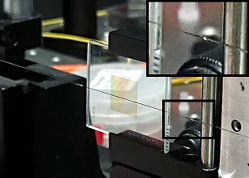
\includegraphics{./messungen/gitter.png}
  \caption{Faser hinter das Beugungsgitter \emph{(Zentrum)}, bereit für die
  Bestrahlung mit dem UV Excimerlaser. Im Detail \emph{(oben rechts)} sieht man
die Grenze zwischen nackte und mit Plastik geschütztes Faser.}
  \label{fig:gitt}
\end{figure}

\begin{figure}[H]
  \centering
  \begin{tikzpicture}
    \begin{axis}[
	title = Spektrum,
	xlabel = Wellenlänge in nm,
	ylabel = Counts,
	%xmin = 5745,
	%xmax = 6206,
      ]
	\addplot[
      	samples=2,
      	%restrict x to domain=5745:6206,
     	] 
	table {./messungen/fbg-01.dat};
    \end{axis}
  \end{tikzpicture}
  \caption{Spektrum nach Bragg-Gitter. Man sieht eine schmale Spalte um 1548
  nm.}
  \label{fig:bragg}
\end{figure}



%\newpage
%\section{Systemdesign sowie Multiplex und Modulationsformate}
%\subsection{unterschiedliche Multiplextechniken}
%\subsection{unterschiedliche Modulationsformate}
%\subsection{Parameter für Systemdesign}
%\paragraph{Leitungsbudget}
%\paragraph{Bitfehlerrate}
%\paragraph{Jitter}
%\paragraph{Augendiagramm}
%\paragraph{Signal-zu-Rausch-Verhältnis}
%\paragraph{Empfängerempfindlichkeit}
%
%\subsection{Versuch}
%Charakterisierung der optischen Übertragungsstrecke:
%Bitfehlerrate in Abhängigkeit von der Dämpfung,
%Augendiagramm in Abhängigkeit von der Dämpfung.

\newpage
\nocite{*}
\bibliographystyle{geralpha}
%\bibliographystyle{plain}
\bibliography{mybib}

\end{document}
